\section{ Turbulence statistics at moderately-high Reynolds numbers} \label{sec:RS_peaks_and_exp}

The streamwise development of the different simulations as well as statistics in different wall-normal profiles are given in appendix \hyperlink{AppA}{A}, where similar conclusions as the ones observed in \cite{bobke2017} for near-equilibrium flows at lower Reynolds numbers are observed and extended to higher $\Rey$ numbers. 

In this section we will present the Reynolds stresses obtained at different streamwise positions since later in section \ref{sec:Spectra} they will be decomposed in their spectral components.

In figure \ref{fig:beta} the Clauser pressure-gradient parameter $\beta=(\delta^*/\tau_w)  (\partial P/\partial x)_{e} $ is shown for the nearly-constant-$\beta$ simulations by \cite{bobke2017}, the current simulation and data obtained in experiments \citep{MTL_expSANMIGUEL} for a similar range of $\Rey_{\tau}-\beta$. Here, $\Rey_{\tau}=u_{\tau}\delta_{99}/\nu$ is the Reynolds number based on friction velocity and $\delta_{99}$ is the $99\%$ boundary-layer thickness, which was calculated by means of the method proposed by \cite{diagnostic_Vinuesa}.

For the following figures, the $Re_{\tau}=500$ profiles (outside the ROI) will be considered to observe effects of different $\beta$, comparing b1.4 with the other near-equilibrium APG simulations at lower $\Rey$. Three additional profiles within the ROI, at $\Rey_{\tau}=\{500, 1000, 1500\}$, will be used to determine the effects of moderate APG at higher $\Rey$ through a comparison with the high-$\Rey$ ZPG. The mean velocity profiles of these cases are shown in figure~\ref{fig:meanU} from Appendix~\hyperlink{AppA}{A}.

\begin{figure}
\centering
% \includegraphics[width=0.6\textwidth]{Statistics/Integ_quant/beta_exp.eps}
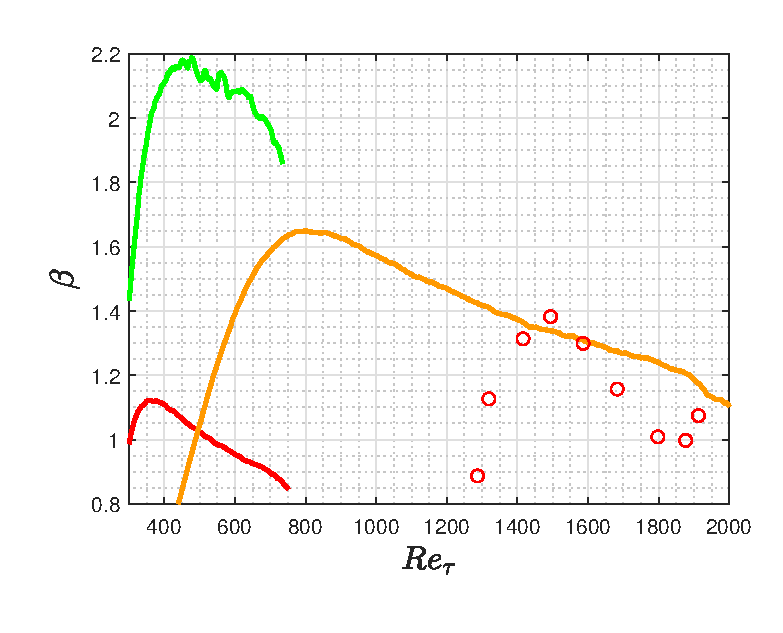
\includegraphics[width=0.6\textwidth]{fig2.eps}
  \caption{Evolution of the Clauser pressure-gradient parameter $\beta$ as a function of the friction Reynolds number $Re_{\tau}$ for three of the simulations Colors: (\protect\orangeline) b1.4; (\protect\redline) b1; (\protect\greenline) b2; (\protect\redcircle) experiments by \cite{MTL_expSANMIGUEL}.}
%   (colors as in table \ref{tab:param}) and the experiments by \cite{MTL_expSANMIGUEL} (represented by red circles).}
\label{fig:beta}
\end{figure}

The inner-scaled Reynolds stresses are shown in figure \ref{fig:RSinner}, and the corresponding profiles in outer scaling can be observed in appendix \hyperlink{AppA}{A}, figure \ref{fig:RSouter}. 
The most noticeable characteristic of these TBLs is that the wall affects each component of the Reynolds-stress (RS) tensor differently. The streamwise component has in general a larger value than the other terms, making it the leading term of the turbulent kinetic energy (TKE). Since at the wall the no-slip condition makes the velocities zero, the RSs also start from a zero level. In the viscous sub-layer the mean velocity gradually increases, together with the velocity fluctuations. 
In the near-wall region, {\it i.e.} at around $y^+\simeq 15$, the streamwise Reynolds stress exhibits the well-known inner peak, while the other fluctuating components are moderately affected by the strong TKE production in this region.

The APG significantly affects the inner peak of $\overline{u^2}^+$, and when this peak is scaled in outer units its magnitude decreases with APG magnitude (see figure \ref{fig:RSouter}a)). Interestingly, the near-wall fluctuations increase slightly with $\beta$ in the other velocity components when scaling in outer units (figure~\ref{fig:RSouter}), a result which is more prominent in the case of $\overline{w^2}$.

In the inner-scaled Reynolds stresses shown in figure \ref{fig:RSinner}, the influence of the APG can be observed in both $\overline{u^2}^+$ and $\overline{w^2}^+$, especially on the latter, from $y^+ \approx 2$ onward. However, the components containing the wall-normal velocity fluctuation are affected farther from the wall, starting at $y^+ \approx 10$ for $\Rey_{\tau}=500$ or even $y^+ \approx 20$ for higher $\Rey$. This behaviour supports the attached-eddy hypothesis on the differing contributions to the Reynolds stresses close to the wall \citep{Townsend_1976, deshpande_2021}, however, the trends are modified by the APG farther from the wall. 
The viscous scaling is appropriate for regions close to the wall, since it properly scales the mean streamwise velocity and the viscous length locates the inner peak of $\overline{u^2}^+$ at $y^+\approx 15$ (see figure \ref{fig:uupeaks_loc}a)). Furthermore, the friction velocity $u_{\tau}$ leads to more similar inner-peak magnitudes from different $\beta$ values than what is obtained using the outer velocity scale $U_{e}$. It is important to recall that the friction velocity is computed from ${\rm d}U / {\rm d} y$, which is the largest term of the near-wall TKE production also in APGs, closely connected with the formation of the inner peak in $\overline{u^2}^+$. The other components of the Reynolds stresses exhibit a better scaling using outer units even close to the wall, as shown in figure \ref{fig:RSouter} from Appendix A. 

 % Reynolds stress in inner units
\begin{figure}
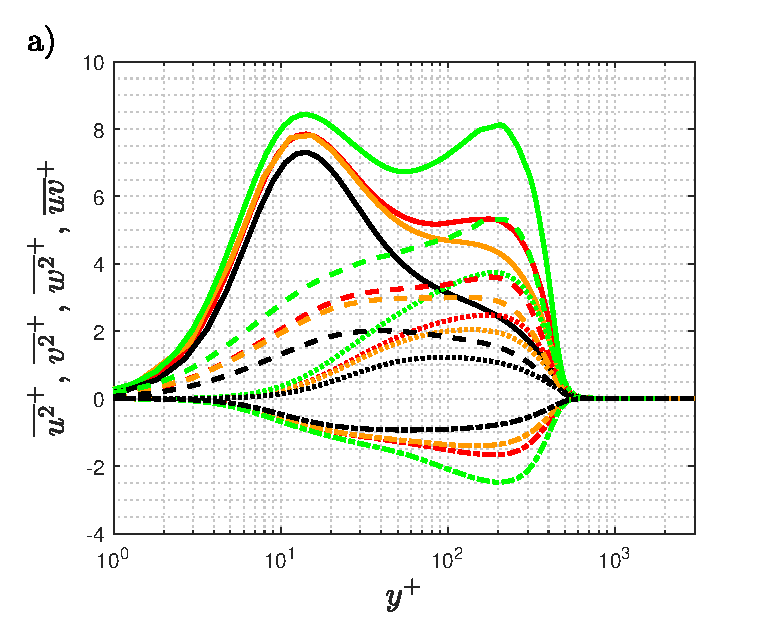
\includegraphics[width=0.49\textwidth]{fig3a.eps}
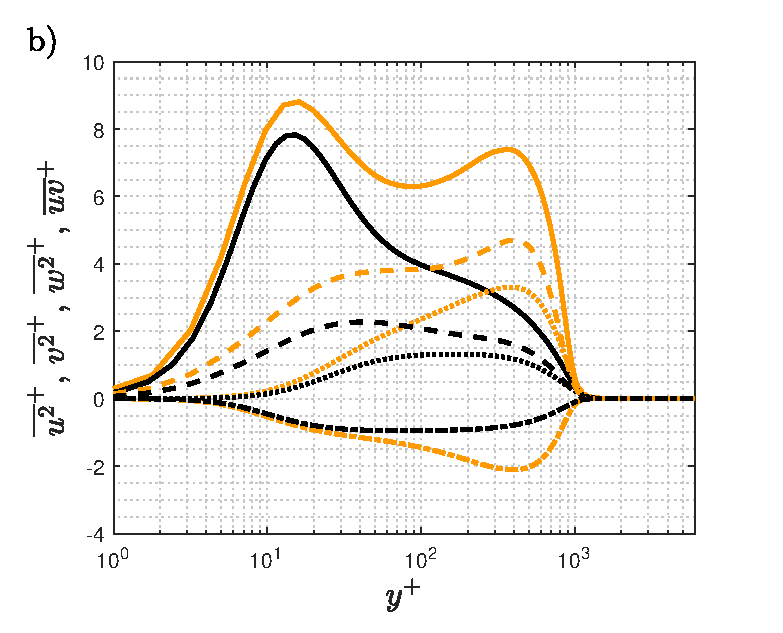
\includegraphics[width=0.49\textwidth]{fig3b.eps} \\
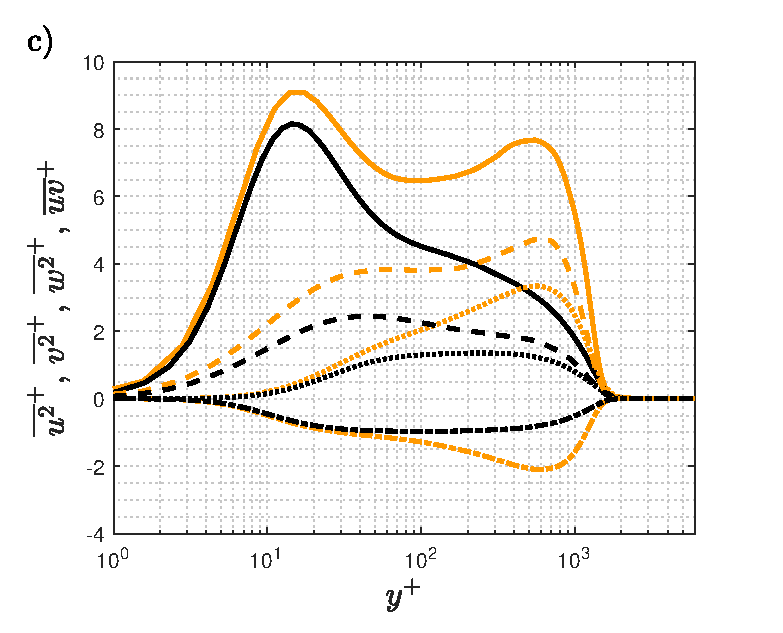
\includegraphics[width=0.49\textwidth]{fig3c.eps}
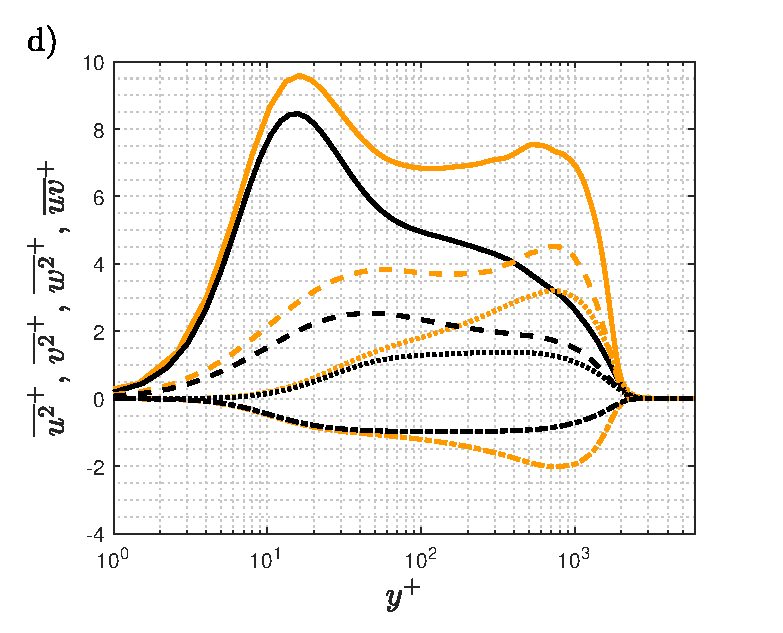
\includegraphics[width=0.49\textwidth]{fig3d.eps}
  \caption{Inner-scaled Reynolds stresses scaled with the friction velocity $u_{\tau}$ at various matched $Re_{\tau}$: a) $Re_{\tau}=500$ where $\beta(Re_{\tau})$ intersects for the simulations b1 and b1.4; b) $Re_{\tau}=1000$ ; c) $Re_{\tau}=1500$ ; d) $Re_{\tau}=2000$. Symbols: (\protect\blackline) $\overline{u^2}^+$; (\protect\blackdotted) $\overline{v^2}^+$; (\protect\blackdash) $\overline{w^2}^+$; (\protect\blackdashdot) $\overline{uv}^+$. Colors and symbols: (\protect\blackline) ZPG; (\protect\redline) b1; (\protect\orangeline) b1.4; (\protect\greenline) b2 as in table \ref{tab:param}.}
\label{fig:RSinner}
\end{figure}

To further study the impact of APG and $\Rey$ on the near-wall and outer peaks, it is important to have fine resolutions around $y^+=15$ and well-converged statistics in the outer region. 

Since the experimental database exhibits some noise, a curve-fit approach was considered around the inner and outer peaks of the streamwise RS to determine their locations, while a simple spline interpolation was employed for the numerical data.

In figure \ref{fig:uupeaks_loc} we show the streamwise evolution of the peak locations, where a clear influence of the APG is observed. Based on our results, an increasing APG magnitude leads to a larger wall-normal location of the inner peak $y^+_{IP}$, a phenomenon which is also observed for higher $\Rey$ at a given constant $\beta$. While for the ZPG case the near-wall-peak location reaches an asymptotic value of around $y^+ \simeq 15$ for $Re_{\tau} >2,000$, the trend in the b1.4 case is currently inconclusive.


\begin{figure}
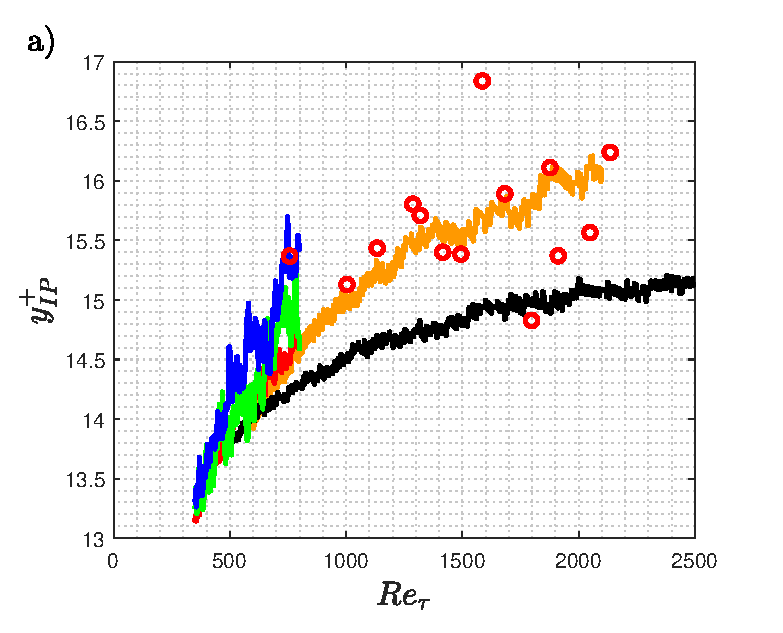
\includegraphics[width=0.49\textwidth]{fig4a.eps}
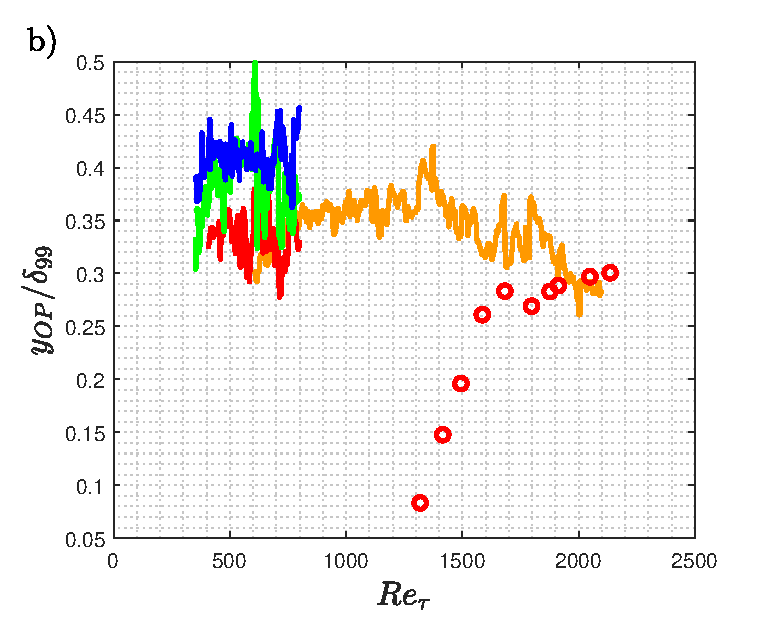
\includegraphics[width=0.49\textwidth]{fig4b.eps} \\
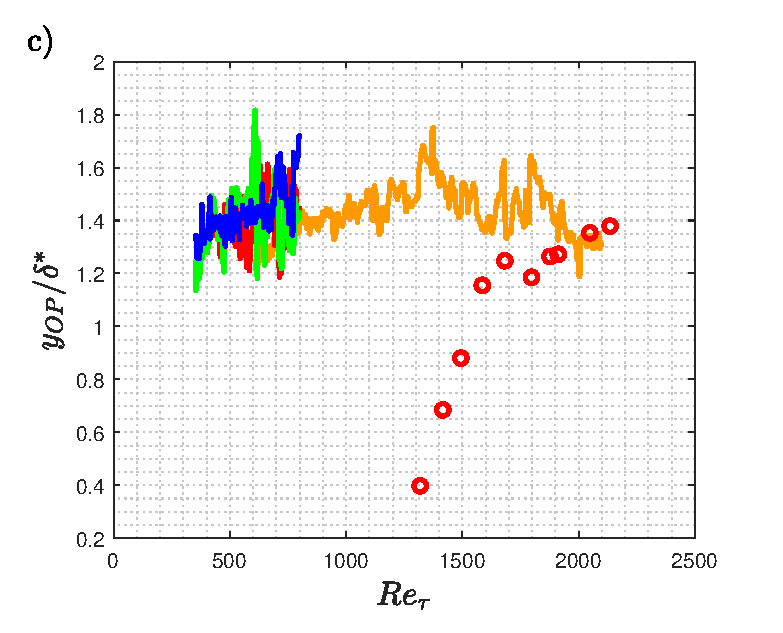
\includegraphics[width=0.49\textwidth]{fig4c.eps}
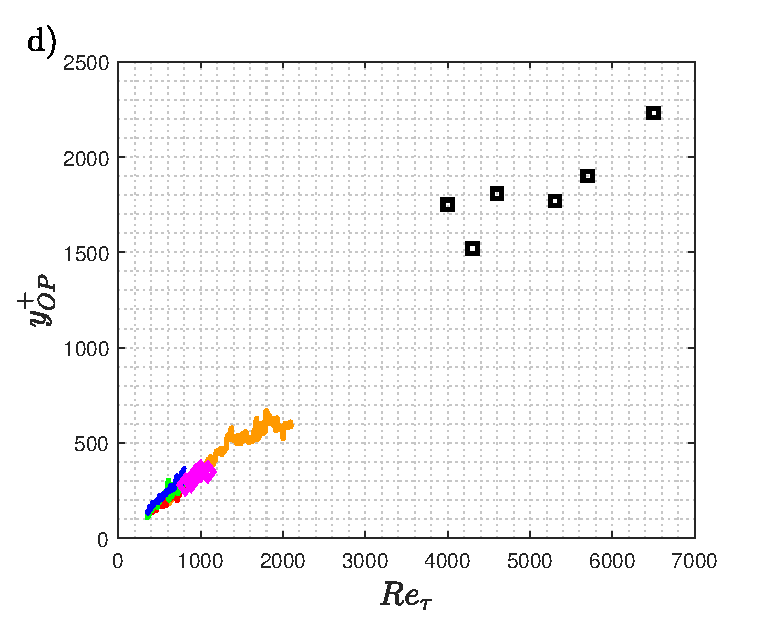
\includegraphics[width=0.49\textwidth]{fig4d.eps}
\caption{Streamwise evolution of the wall-normal location of the inner and outer peaks of the streamwise Reynolds stress profiles. a) Inner-scaled position of the inner peak $y_{IP}^+$; b) and c) outer-peak location ($y_{OP}$) scaled with $\delta_{99}$ and $\delta^*$, respectively; d) inner-scaled outer-peak location $y^{+}_{OP}$. Colors: (\protect\blackline) ZPG; (\protect\orangeline) b1.4; (\protect\redline) b1; (\protect\greenline) b2; (\protect\blueline) m16; (\protect\magentaDiamond) $\beta=1$ DNS data from \cite{Kitsios2016}; (\protect\redcircle) experiments by \cite{MTL_expSANMIGUEL}; (\protect\blackSquare) experiments by \cite{skare_krogstad_1994}.}
\label{fig:uupeaks_loc}
\end{figure}
\begin{figure}
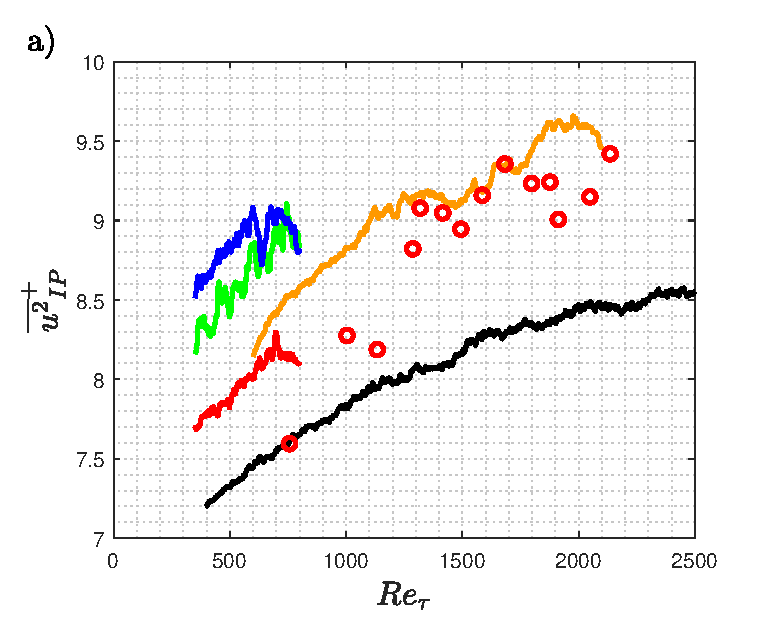
\includegraphics[width=0.49\textwidth]{fig5a.eps}
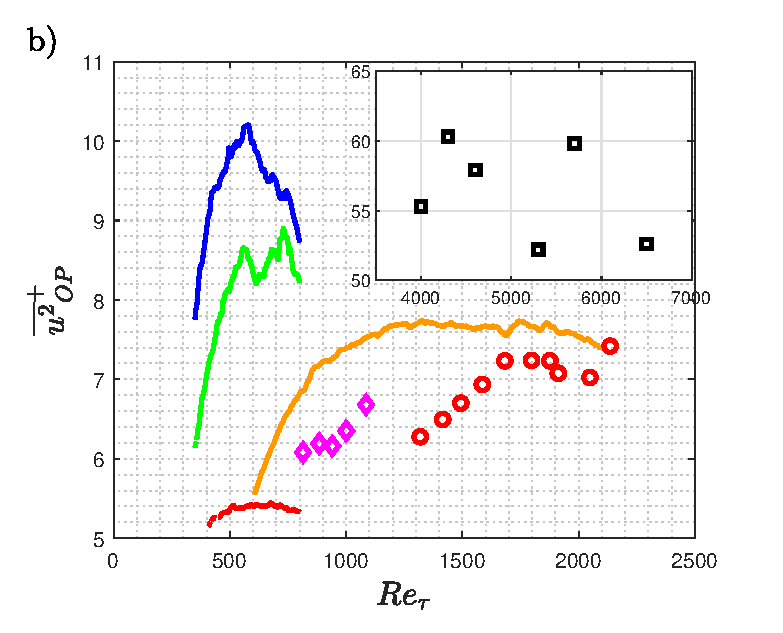
\includegraphics[width=0.49\textwidth]{fig5b.eps}\\
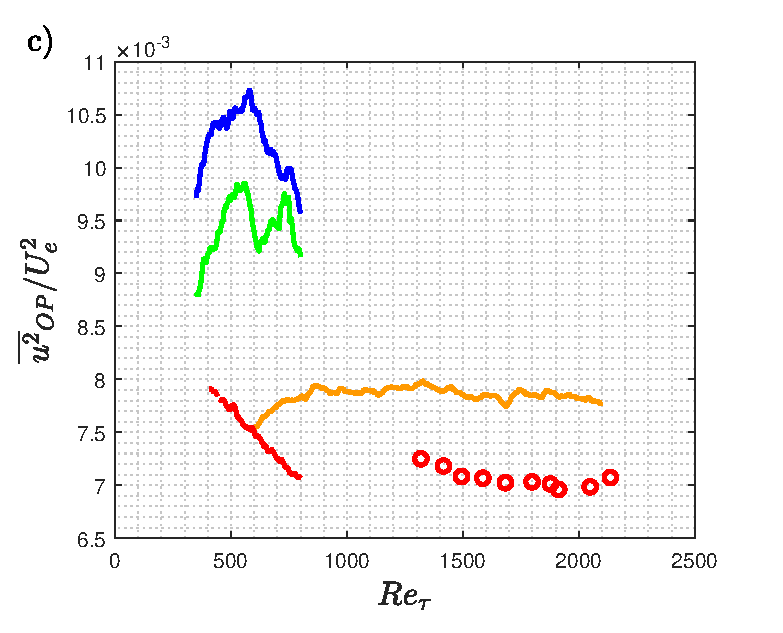
\includegraphics[width=0.49\textwidth]{fig5c.eps}
  \caption{Streamwise evolution of the magnitude of the inner and outer peaks of the streamwise Reynolds stress profiles. a) Inner-scaled magnitude of the inner peak $\overline{u^2}^+_{IP}$; b) and c) outer-peak magnitude ($\overline{u^2}_{OP}$) scaled in inner and outer units, respectively. Colors: (\protect\blackline) ZPG; (\protect\orangeline) b1.4; (\protect\redline) b1; (\protect\greenline) b2; (\protect\blueline) m16; (\protect\magentaDiamond) $\beta=1$ DNS data from \cite{Kitsios2016}; (\protect\redcircle) experiments by \cite{MTL_expSANMIGUEL}; (\protect\blackSquare) experiments by \cite{skare_krogstad_1994}. }
\label{fig:uupeaks_val}
\end{figure}

Figure \ref{fig:uupeaks_loc}b) shows the outer-peak location $y_{OP}$ of $\overline{u^2}$, scaled with the $99\%$ boundary-layer thickness, and our results indicate that the curve reaches a slightly decaying trend with $\Rey$ in the b1.4 case. 
Furthermore, comparison with the other cases indicates that the values of $y_{OP}/\delta_{99}$ are clearly affected by $\beta$, with stronger APGs leading to larger values of the outer-peak location. Note that although the value of $\beta$ is approximately the same in the b1 simulation and in the experiment, the former is at a much lower Reynolds number, and therefore this case is expected to perceive a more intense effect of the APG. This would explain that the outer-peak location is slightly farther away from the wall in the b1 case than in the experiment.
Figure \ref{fig:uupeaks_loc}c) shows the outer-peak location of $\overline{u^2}$ scaled with the displacement thickness $\delta^*$. The low-$\Rey$ simulations exhibit a similar slowly-growing trend for the various $\beta$ cases, with an average value of around $y_{OP}/\delta^* = 1.4$. The b1.4 case appears to reach an approximately constant state at higher $\Rey$, also around 1.4, a result consistent with that reported by \cite{Sanmiguel_PRF} for the experimental data (despite the noise present in the measurements).

The inner-scaled location of the outer peak present in the DNS by \cite{Kitsios2016} and the experiments by \cite{skare_krogstad_1994} are also shown in figure \ref{fig:uupeaks_loc}d). The outer-peak location of the $\beta=1$ DNS by \cite{Kitsios2016} continues the trend defined by the b1 LES at lower $\Rey$ and lies below the line of the b1.4 LES. The values of the near-equilibrium experimental data by \cite{skare_krogstad_1994} at a much higher $\Rey$ and $\beta \approx 20$ appear to be consistent with the linear trend of $y_{OP}^+$ established by the lower-$\Rey$ data.


The magnitudes of the inner ($\overline{u^2}_{IP}$) and outer ($\overline{u^2}_{OP}$) peaks of the streamwise RS are shown in the different panels of figure \ref{fig:uupeaks_val}.
In panel a) it is possible to see the Reynolds-number evolution of the inner-scaled inner peak ($\overline{u^2}_{IP}^+$) for the various APGs, as well as that of the ZPG TBL, which is well documented in the literature \citep{E-AmorZPG, Marusic_1997_ZPG}. While it is unclear what the behavior will be for the APG cases at higher $\Rey$, our data indicates that the inner-scaled near-wall peak increases with APG magnitude. The trend from the experiment exhibits more scatter, but it appears to be in qualitative agreement with that of the b1.4 case. Note that, although the inner peak in inner scaling increases with $\beta$, it actually decreases in outer scaling for stronger APGs, as can be observed in figure \ref{fig:RSouter}.
The outer-peak value increases with $\beta$ using inner scaling, as shown in figure \ref{fig:uupeaks_val}b), and also in outer scaling with $U_e$, as illustrated in figure \ref{fig:uupeaks_val}c). In both panels, the trends are approximately constant with $\Rey_{\tau}$, where $U_{e}$ yields a reasonably flat curve even at lower Reynolds numbers. 


In figure \ref{fig:uupeaks_val}b) the location of $\overline{u^2}^+$ for the $\beta=1$ DNS by \cite{Kitsios2017} and the b1 LES exhibit small differences probably associated with the different flow histories at low Reynolds numbers.
The experimental data by \cite{skare_krogstad_1994} exhibits a larger uncertainty and dispersion of the values, but an approximately-constant trend in $\overline{u^2}^+$ can be observed.

An unexpected trend is observed in figure \ref{fig:uupeaks_val}c) for the b1 simulation, a fact that could be attributed to the relatively low outer-peak values in this simulation.




%*********************************************************************************
% Experiments in MTL
%*********************************************************************************
\subsection{Comparison with experiments} 

The range of Reynolds numbers achieved in the b1.4 case allows for a direct comparison of the statistics with the experimental results by \cite{MTL_expSANMIGUEL}, where we selected two cases with matching $\beta$ and $\Rey_{\tau}$ conditions. As shown in  figure \ref{fig:beta}, the flow history of this database differs from that of the b1.4 case, a fact that will be taken into account when comparing the data.

\begin{figure}
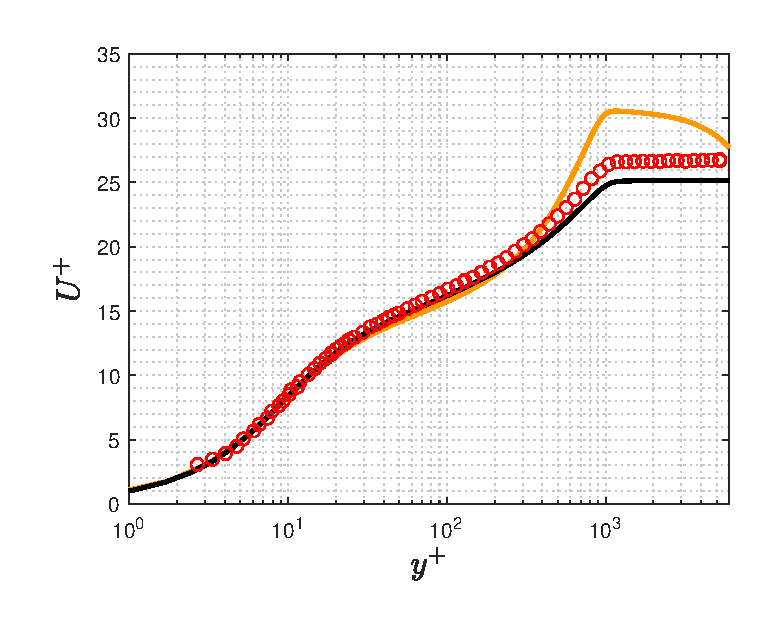
\includegraphics[width=0.49\textwidth]{fig6a.eps}
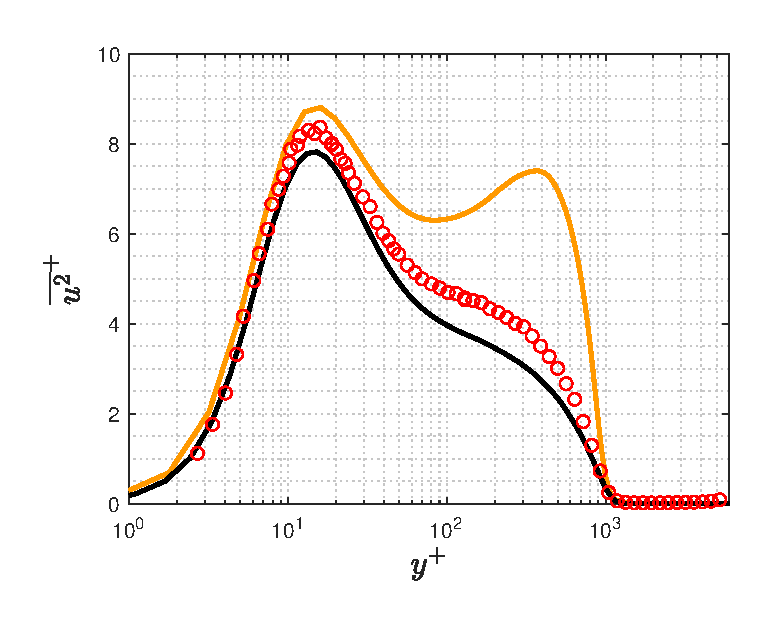
\includegraphics[width=0.49\textwidth]{fig6b.eps}
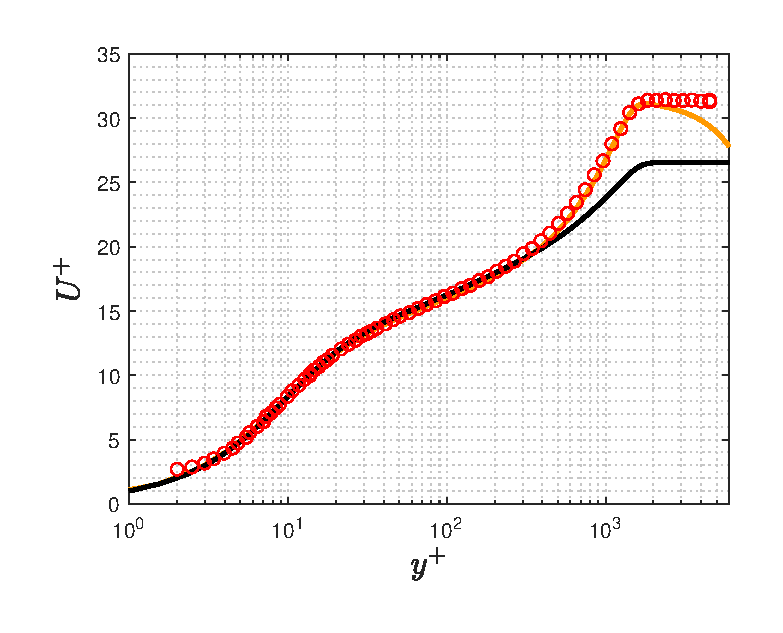
\includegraphics[width=0.49\textwidth]{fig6c.eps}
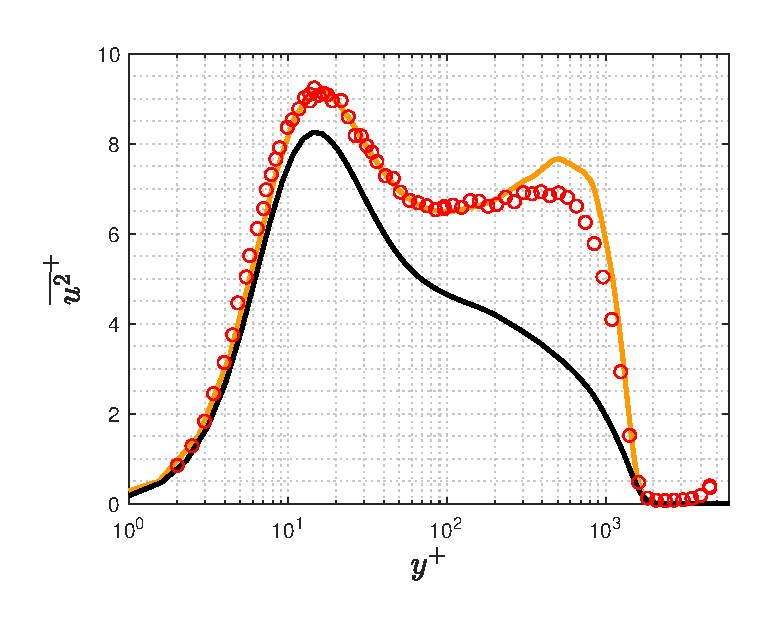
\includegraphics[width=0.49\textwidth]{fig6d.eps}
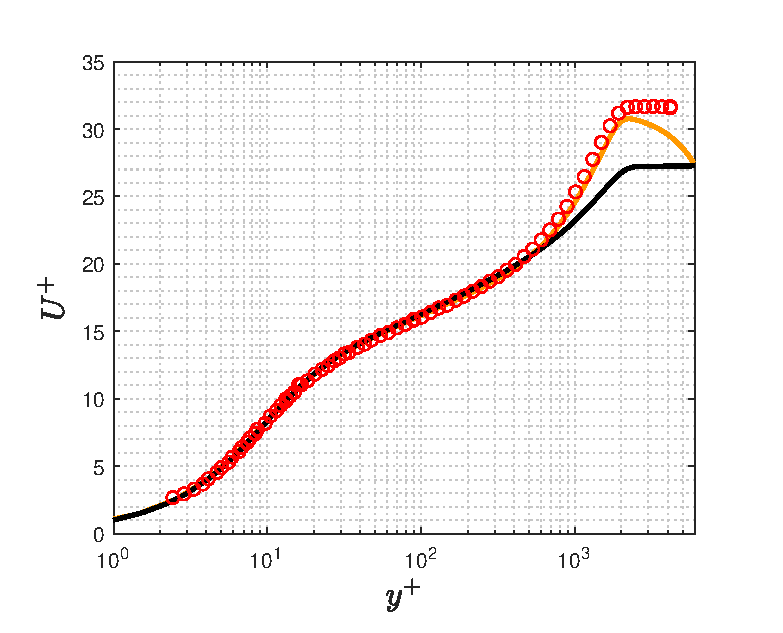
\includegraphics[width=0.49\textwidth]{fig6e.eps}
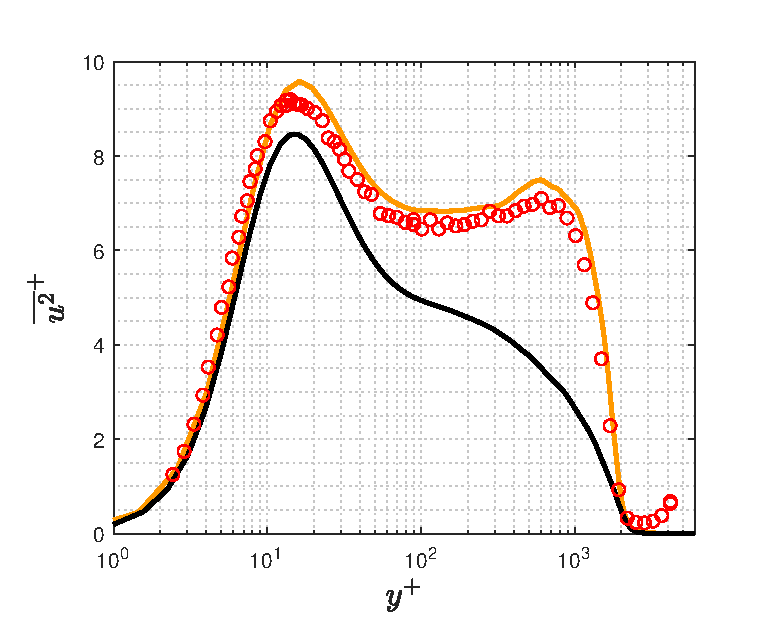
\includegraphics[width=0.49\textwidth]{fig6f.eps}
\caption{Mean velocity (left column) and streamwise Reynolds stress (right column) scaled in viscous units as a function of the inner scaled wall-normal distance. The Reynolds numbers from top to bottom are $Re_{\tau}=\{1004, 1586, 2049\}$. The black solid line represents the ZPG by \cite{E-AmorZPG}, the orange line is the present b1.4 simulation and the red circles represent the experimental data by \cite{MTL_expSANMIGUEL}.}
\label{fig:experimentsMTL}
\end{figure}
%  Colors: (\protect\blackline) ZPG; (\protect\orangeline) b1.4; (\protect\redcircle) experiments by \cite{MTL_expSANMIGUEL}.

Three different profiles have been chosen in figure \ref{fig:experimentsMTL} to show the mean streamwise velocity and the streamwise Reynolds stress from the simulation and the experiment at matching $\Rey_{\tau}$. In the first row ($\Rey_{\tau}=1004$) the experimental TBL has a very low $\beta=0.3$, and it is very close to the ZPG, with small differences in the near-wall peak of $\overline{u^2}^+$ and a growing energy in the outer region of the TBL.
Here the simulation has a larger value of $\beta=1.6$, and it exhibits the most relevant features of APGs, including a prominent outer peak in $\overline{u^2}^+$.
In the middle row ($\Rey_{\tau}=1586$) the experimental data and the numerical simulation b1.4 exhibit the same  $\beta \simeq 1.4$. While the mean velocity profiles and the near-wall region of $\overline{u^2}^+$ is in good agreement in both cases, the simulation exhibits a larger fluctuation peak. This is due to the effect of flow history \citep{bobke2017, tanarro_2020}, but it is interesting to note that while the simulation is subjected to a mildly decaying $\beta(x)$ curve, the APG is rapidly increasing in the experiment. This implies that the smaller scales adapt more quickly to the local pressure gradient, while the larger scales require a longer streamwise distance.  
Finally, the higher Reynolds-number profile ($\Rey_{\tau}=2049$), where both TBLs have a value of $\beta \simeq 1.1$, exhibits a better collapse in both inner and outer peaks of $\overline{u^2}^+$, as well as in the mean velocity $U^+$.
This implies that, despite the different flow histories upstream, the two TBLs have been exposed to a similar PG magnitude for a sufficiently long streamwise distance such that their local turbulence features converge. Several profiles have been compared for $\Rey_{\tau}>1586$, and the best agreement between simulation and experiment is obtained for $\Rey_{\tau}=2049$. Upstream of this position the outer-peak value of the experimental data is still developing towards the value of the b1.4 case. The streamwise distance between the profiles at $\Rey_{\tau}=1586$ and 2049, which are subjected to a similar $\beta$ history, is around $11 \overline{\delta_{99}}$ for both simulation and experiment, where $\overline{\delta_{99}}$ is the average boundary-layer thickness between those profiles. A similar albeit lower of around $7\overline{\delta_{99}} $ was reported by \cite{bobke2017} for m16 simulation to converge towards b2 simulation at $\Rey_{\tau}=786$. One possible explanation for the longer distance reported here may be the higher Reynolds number, in which the large scales may require longer streamwise lengths to adapt to a particular pressure-gradient condition.

The APG in the simulation is achieved through a free-flow boundary condition, the turbulence is achieved through a tripping, therefore, the turbulence is confined inside the boundary layer with the Reynolds stresses being negligible outside of it. The experiments are performed inside a wind tunnel, the APG is imposed through changes in the geometry of the upper wall where another turbulent boundary layer develops. Even though the methods to establish the two APG TBLs are different, the results are remarkably similar. 
While the region outside of the boundary layer in the wind tunnel can be seen as the flow in the core of a channel where the mean $U$ does not exhibit a significant change, the free-flow APG condition has a negative $\partial{U}/\partial{y}$. This gradient, even if small, is present over a large distance in $y$, and when the mean profile is represented in a logarithmic scale it gives the impression of a drastic reduction of the mean velocity for $y>\delta_{99}$.
This comparison between numerical simulation and experiments shows a satisfactory collapse, and thus validates the high-Reynolds-number region of this numerical simulation.
